\chapter{پیاده‌سازی}
در بخش قبلی معماری کلی سیستم و ماژول‌های موردنیاز برای پیاده‌سازی سیستم ردیابی را بیان و به صورت اجمالی معرفی کردیم. در این فصل به چگونگی قرار گرفتن و ارتباط بخش‌های مختلف می‌پردازیم و پیاده‌سازی سیستم را توضیح خواهیم داد.


سیستم ردیابی طراحی شده در این پروژه از ماژول \lr{Arduino uno} و ماژول \lr{SIM808} که شامل آنتن \lr{GSM} و \lr{GPS} می‌باشد، برای ردیابی استفاده می‌کند. هسته اصلی این پروژه میکروکنترلر آردوینو می‌باشد. موقعیت جغرافیایی شی تویط آنتن \lr{GPS} دریافت شده و سپس این اطلاعات با استفاده از تکنولوژی \lr{GSM} به وب سرور فرستاده می‌شود. برای مشاهده کردن و ردیابی شی بر روی نقشه، یک برنامه کاربردی تحت وب توسعه داده شده است. این برنامه کاربردی به زبان \lr{PHP}، \lr{HTML} نوشته شده و از نرم‌افزار \lr{WampServer} برای اجرای آن استفاده می‌شود.
 
 
در ابتدا ماژول \lr{Sim808} برای گرفتن موقعیت مکانی از ماهواره مقداردهی اولیه می‌شود. تنظیمات اولیه این دستگاه با استفاده از دستورات \lr{AT} انجام می‌شود. با متصل کردن آنتن \lr{GPS} این ماژول قادر خواهد بود مختصات مکانی را از ماهواره دریافت کند. سپس تنظیمات مربوط به شبکه \lr{GPRS} انجام می‌شود.


آنتن‌های \lr{GSM} و \lr{GPS} به ماژول \lr{SIM808} متصل می‌شوند. برد آردوینو و ماژول \lr{SIM808} دارای پین اتصال به زمین مشترک هستند. برنامه نوشته شده به زبان \lr{C} بر با استفاده از نرم‌افزار \lr{Arduino IDE} روی برد آردوینو آپلود می‌شود.
\\
در شکل ۴-۱ نحوه اتصال ماژول‌های مختلف در سیستم ردیابی نشان داده شده است:
\begin{figure}[!h]
	\centerline{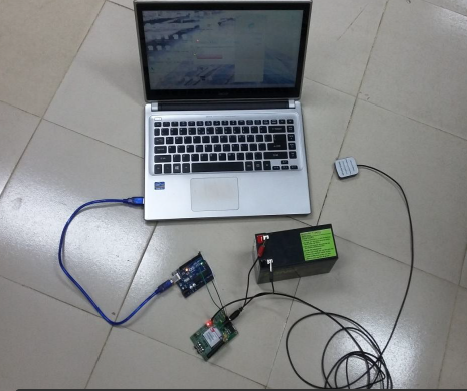
\includegraphics[width=.6\textwidth]{design-system}}
	\caption{سیستم ردیابی طراحی شده}
\end{figure}
\section{بررسی عملکرد سیستم ردیابی}
همانطور كه گفته شد، قسمت سخت‌ افزاری سیستم ما از چهار ماژول \lr{SIM808}، گیرنده جی‌اس‌ام، گیرنده جی‌پی‌اس و میکروکنترلر آردوینو تشکیل شده است. در اين قسمت، پياده‌سازي سيستم طراحی شده، شيوه ارتباط اجزای مختلف و كد پياده‌سازي شده را توضيح خواهیم داد.
\subsection{بررسی عملکرد مدار}
پيش از پرداختن به ماژول‌ها و شيوه اتصال آن‌ها، لازم است شيوه عملكرد ميكروكنترلر سيستم و نحوه پردازش اطلاعات را در فلوچارتي مشاهده كنيم. عملكرد كلي سيستم در بخش قبل توضيح داده شد. اكنون با ارئه فلوچارتي درباره الگوريتم پياده‌سازي شده می‌توانیم درك بهتري نسبت به روند كار در مدار سخت‌افزاری طراحی شده و كد نوشته شده براي آن داشته باشيم.
فلوچارت شكل ۴-۲ روند كلي كد پياده‌سازي شده بر روي آردوینو را نمايش می‌دهد.
\begin{figure}[!h]
	\centerline{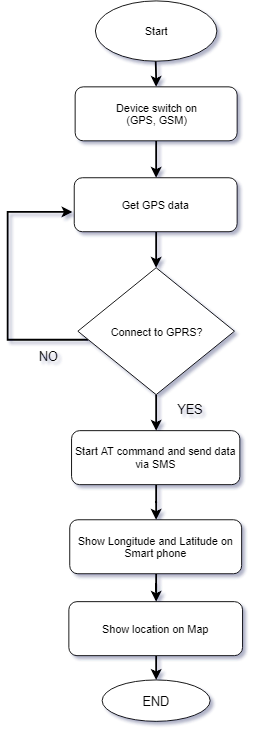
\includegraphics[width=.5\textwidth]{tracking-flowchart}}
	\caption{عملکرد کد پیاده‌سازی شده بر روی آردوینو \cite{Rahman2016,Alshamsi,Hazza}}
\end{figure}

\\
در ابتدای کار برای تست سیستم طراحی شده، آنتن جی‌پی‌اس به ماژول \lr{SIM808} متصل می‌شود تا موقعیت مکانی (طول و عرض جغرافیایی) شی را از ماهواره دریافت کند. برای انجام این کار از نرم افزار \lr{Arduino IDE} برای پروگرم کردن کد نوشته شده بر روی برد آردوینو استفاده می‌شود.
در فلوچارت شکل ۴-۳ نحوه کار \lr{GPS} را نشان داده شده است.
\begin{figure}[!h]
	\centerline{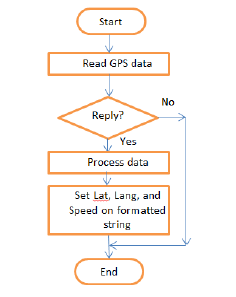
\includegraphics[width=.6\textwidth]{gps-flowchart}}
	\caption{فلوچارت خواندن اطلاعات \lr{GPS} \cite{ElShafee2013}}
\end{figure}